\subsection{Emerging Advancements in Reconfiguration Technologies}
\subsubsection{MOSAR Project Outcomes}
The MOSAR project has achieved several significant outcomes to date:
\begin{itemize}[]
	\item Development of a standardized module framework utilizing the HOTDOCK adapter.
	\item Design and fabrication of a walking manipulator arm.
	\item Establishment of a related system architecture for remote control of the manipulator arm.
	\item Successful ground demonstration showcasing the manipulator arm's capabilities to move and connect modules.
	
\end{itemize}
At this stage, the MOSAR demonstrator could theoretically perform reconfiguration in orbit but currently requires manual transmission of reconfiguration instructions to the craft. Further work is needed to enable automated functionality, including:
\begin{itemize}[]
	\item Automatic determination of a desired module configuration to meet mission requirements.
	\item Automated computation of manipulator instructions necessary to reconfigure the craft from one configuration to another.
	
\end{itemize}
The following review of automated reconfiguration literature will focus on identifying the best methods for the computation of manipulator instructions.

\subsubsection{Automated Reconfiguration}
Automatic planners, algorithms that find a solution for which sequence of operations must be accomplished to achieve a specified goal, have been an area of development attracting wide-spread interest since the earliest days of robotics. Currently there are many different types of automatic planning techniques available. They encompass a large set of algorithmic requirements which trend towards purely discrete or purely continuous search space characteristics. The development of “Hybrid” automated planning approaches with search space characteristics that are not purely discrete or continuous, especially Task and Motion Planning (TAMP) algorithms, represent an area of study of which solutions are considered the most computationally difficult in theory \cite{Deshpande2020}. Consequently, the application of automated planning algorithms to robotic assembly of modular satellites is a very recent development in which little work has been published that implements automatic reconfiguration algorithms while fully considering the range of real-world physical restraints and limitations presented by usage of a mobile manipulator arm in a low-gravity environment.
\begin{figure*}[!t]
	\centering
	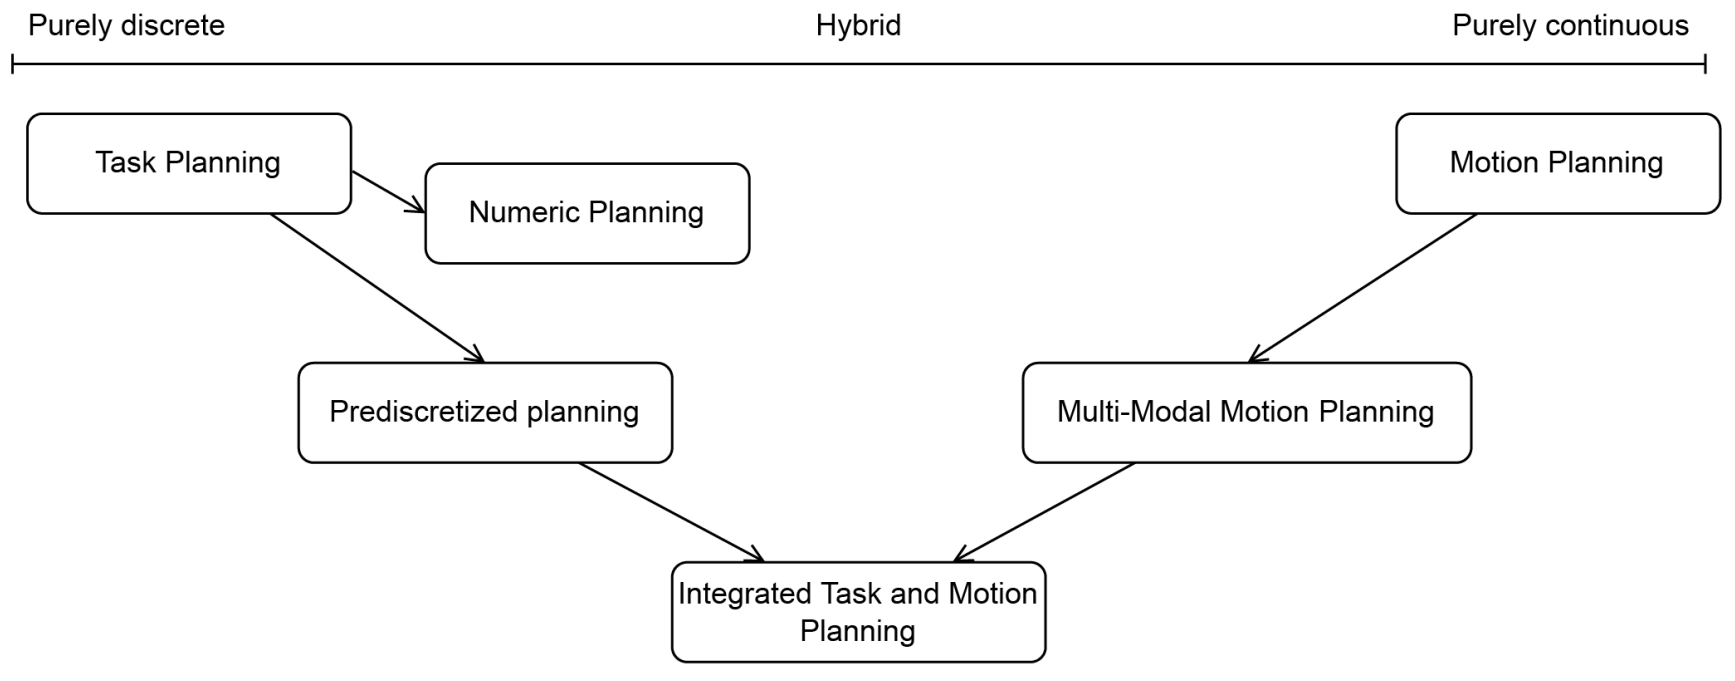
\includegraphics[width=\textwidth]{planningtaxonomy}
	\caption{Taxonomy of automated planning approaches based on their search spaces’ characteristics. Image from \cite{huang2023algorithmic}}
	\label{taxonomy}
\end{figure*}
\subsubsection{Motion and Manipulation Planning}
Motion Planning is finding solutions to move a robot “from one configuration to another configuration without colliding with the objects in the world” \cite{huang2023algorithmic}. It involves searching for paths within the robots reach which is a continuous configuration space limited by dimensions represented by the joints of the robot. These collision-free paths are important for robot motion but do not by themselves allow the robot to interact with the world. Further planning must be implemented to allow manipulation of objects through manipulation planning (known as Multi-Modal Motion Planning).
\\\\
Due to the increased complexity of the problem presented by manipulation planning, the problem is best broken down into a hybrid discrete-continuous search problem of “selecting a finite sequence of discrete action types (e.g. which objects to pick and place), continuous action parameters (such as object poses to place and grasps), and continuous motion paths” \cite{huang2023algorithmic}.
\subsubsection{Task Planning}
While Motion and Manipulation planning are seen as problems mainly within the robotics field, planning within large discrete domains such as in problems presented by task planning has been more deeply researched within the artificial intelligence (AI) community \cite{ghallab2004automated}. Task planning (also known as Action planning) referring to deducing a composition of symbolic actions to achieve a high-level goal (e.g. computing a sequence of actions required to stack boxes in a specified order). The discrete nature of the problem makes it particularly suitable for many machine learning techniques which have particularly advanced in recent years.
\pagebreak
\subsubsection{Task and Motion Planning}
Current research in task and motion planning (TAMP) primarily aims to combine the robotics solutions for manipulation planning under physical constraints with the usually unrestricted AI approach to task planning. With the goal of deriving automated planning systems capable of reasoning symbolically with discrete “high-level” robotic action sets while geometrically taking into account continuous “low-level” robotic motion planning and restrictions. To date, several papers have developed algorithms for similar TAMP problems to the scenario of modular satellite reconfiguration that unfortunately are not compatible due to the method of module mobility, but act as a proof of concept that a solution is possible \cite{1013348, 8206101, 7091046}.

\subsubsection{Related Work}
The 2010 Intelligent Building Blocks for On-Orbit Satellite Servicing and Assembly (IBOSS) project \cite{iBOSS} by DLR provided many advances in the area of satellite modularization with the development of standardised building blocks and interfaces \cite{iBossPaper}. Simple task planning techniques were implemented using Hierarchical task network (HTN) planning to produce high-level mobile arm instruction sets to then be verified through inverse kinematic checks and motion planning. This implementation solved the discrete and continuous planning problems separately, which simplified the problem however does not allow the separate systems to properly integrate. The system was not capable of efficiently solving more difficult tasks of identifying were solutions where not feasible.
\\\\
Alternatively, another approach was taken here \cite{8581406} through the implementation of the melt-grow algorithm \cite{773975}. The physical restraints of the robot were not including in the reconfiguration planning stage of the system, effectively reducing the problem to task planning. This reduces complexity though can only be achieved due to the behaviour of the melt-grow algorithm, which deconstructs (melts) the initial module configuration into chains of modules defined as the intermediate configuration, seen in configuration d in figure \ref{meltgrow}, before then reconstructing (growing) the modules into the expected configuration. The system then does not need to consider whether a move is possible for the mobile arm through manipulation planning as due to the algorithms inclusion of an intermediate state between the melting and growing operations, the algorithm essentially reconstructs the satellite instead of modifying the current state, all required moves are possible for the mobile manipulator and simply require motion planning.
\begin{figure*}[!t]
	\centering
	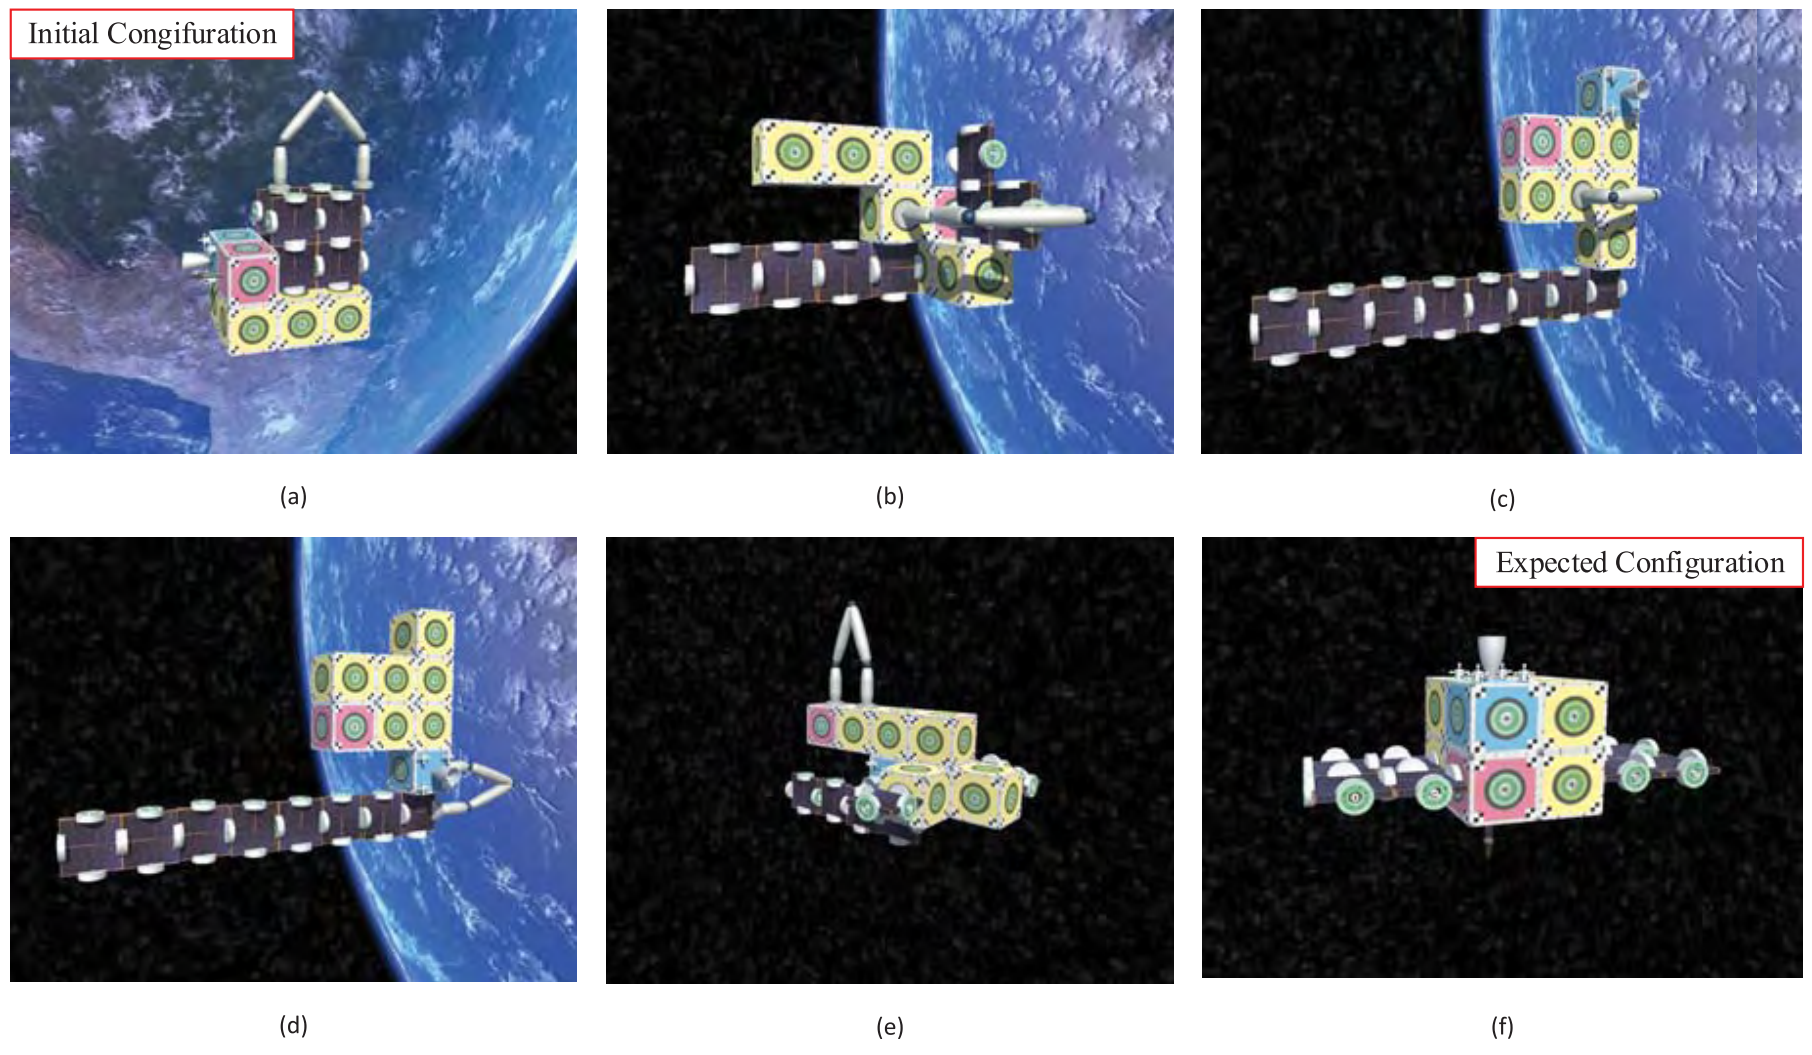
\includegraphics[width=\textwidth]{meltgrow}
	\caption{Melt-Grow algorithm simulation results. Image from \cite{8581406}}
	\label{meltgrow}
\end{figure*}
While proven to work, this method is shown to be highly inefficient for the mobile manipulator, especially as the number of modules increases in the system. Though, the paper \cite{8581406} suggests this could be offset by the inclusion of additional manipulators which would consequently increase construction and operational costs.
\\
More recent research has taken inspiration from these previous works to propose a comprehensive Task and Motion Planning (TAMP) problem solver \cite{9438257} to intrinsically include the robot constraints into the system.  The system, seen in figure \ref{feedbackSystem}, includes a logic layer, a physical layer, and a feedback system. Where the logic layer acts as a task planner finding a semantic solution by considering the solution as a sequence of states, with module movements defining the transition between states. A graph is developed to represent the possible states where nodes are system states and edges represent module movements which are verified by the physical layer which provides manipulation planning results through the feedback system. Using this graph the shortest and hence most efficient set of operations to reconfigure the system into the desired state can be identified. The removal of the intermediate configuration present in the melt-grow algorithm improves the efficiency of the solution set of operations, especially as the number of modules in the system increases, requiring less movement from the mobile manipulator.
\begin{figure*}[!t]
	\centering
	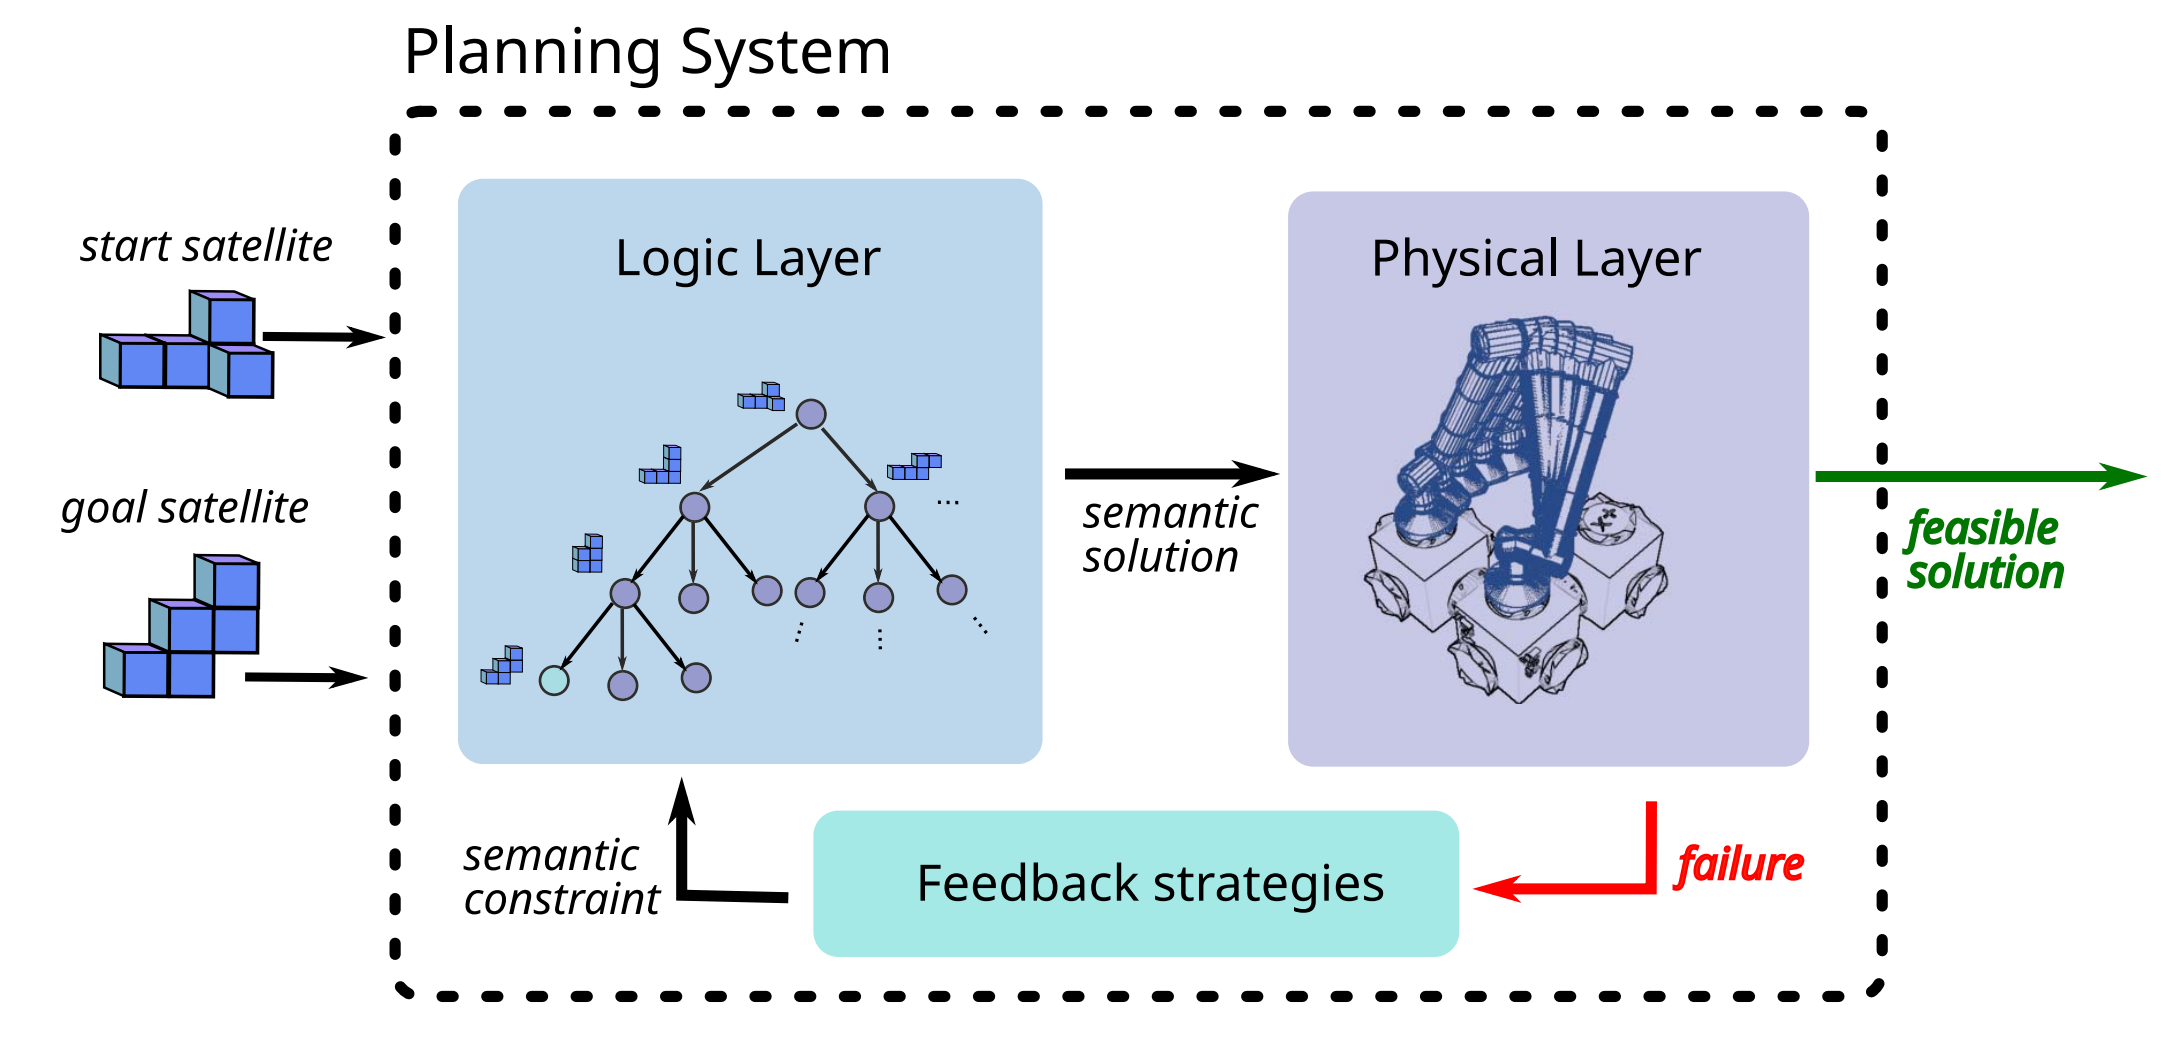
\includegraphics[width=\textwidth]{feedbackSystem}
	\caption{“Architecture of the autonomous robot planning system. The system receives as inputs the start and goal satellite configurations, and iterates between the logic and physical layer until a solution is found.” Image and text from \cite{9438257}}
	\label{feedbackSystem}
\end{figure*}
The paper notes “the goal of this work was not to set a baseline for planning problems in terms of absolute times, but to demonstrate the usefulness of integrating feedback from the physical layer on the logic layer.” \cite{9438257}, suggesting that there is an opportunity for further research into the components of the planning system and the related feedback strategies to prepare the system for space applications.